\documentclass[a4paper]{article}

%====================== PACKAGES ======================

\usepackage[english]{babel}
\usepackage[utf8]{inputenc}
%pour gérer les positionnement d'images
\usepackage{float}
\usepackage{amsmath}
\usepackage{bm}
\usepackage{graphicx}
\usepackage[colorinlistoftodos]{todonotes}
\usepackage{url}
%pour les informations sur un document compilé en PDF et les liens externes / internes
\usepackage{hyperref}
%pour la mise en page des tableaux
\usepackage{array}
\usepackage{tabularx}
%pour utiliser \floatbarrier
%\usepackage{placeins}
%\usepackage{floatrow}
%espacement entre les lignes
\usepackage{setspace}
%modifier la mise en page de l'abstract
\usepackage{abstract}
%police et mise en page (marges) du document
\usepackage[T1]{fontenc}
% \usepackage[top=3cm, bottom=3cm, left=3cm, right=3cm]{geometry}
% Pour les galerie d'images
\usepackage{subfig}
\usepackage{amsmath}
\usepackage{amssymb}
\usepackage{caption}
\usepackage{epsfig}
\usepackage{minitoc}
\usepackage{subcaption}
\newcommand{\eq}{\overline}
\newcommand{\barre}{\widetilde}
\newcommand{\R}{\mathbb{R}}
\usepackage{enumitem}
\setlength{\emergencystretch}{4em}
%====================== INFORMATION ET REGLES ======================

%rajouter les numérotation pour les \paragraphe et \subparagraphe



%======================== DEBUT DU DOCUMENT ========================

\begin{document}

%régler l'espacement entre les lignes
\newcommand{\HRule}{\rule{\linewidth}{0.5mm}}

%page de garde
\begin{titlepage}
\begin{center}

% Upper part of the page. The '~' is needed because only works if a paragraph has started.

\LARGE \textsc{2EL1740: Algèbre \& Cryptologie}

\vspace{0.2cm}

\Large \textsc{CentraleSupélec - 2A}

\vspace{0.3cm}

% Title
\HRule \\[0.4cm]

{\huge \bfseries Challenge 4\\
[0.2cm]}

\HRule \\[0.4cm]

\vspace{2cm}

\textsc{\today}

\vspace{2cm}


\includegraphics[width=0.4\columnwidth]{./logo}~\\[3cm]

% Author and supervisor
\begin{minipage}{0.4\textwidth}
\begin{spacing}{1.125}
\begin{center}
    Raphaël \testsc{PAIN DIT HERMIER}\\
    Alexis \testsc{LOMBARD-GAILLARD}\\
    Edward \testsc{LUCYSZYN}
\end{center}
\end{spacing}
\end{minipage}

\vfill

\end{center}
\end{titlepage}

%page blanche
%\newpage
%~
%ne pas numéroter cette page
\thispagestyle{empty}


\tableofcontents
\thispagestyle{empty}
%ne pas numéroter le sommaire

%\newpage

%espacement entre les lignes d'un tableau
\renewcommand{\arraystretch}{1.5}

%====================== INCLUSION DES PARTIES ======================

~
\thispagestyle{empty}
%recommencer la numérotation des pages à "1"
\newpage

\section{Introduction}

\hspace{0.8cm} Knowing how to solve the equations of acoustic and electromagnetic waves can help solve many of today's challenges, such as limiting noise in an aircraft engine or insulating a building from noise pollution.\\ \\
Solving these equations analytically can quickly become impossible. That's why you need to know how to solve them numerically. Throughout this report, we'll look at methods for controlling, analyzing and using the mesh of a finite-difference method, for example.\\ \\
First of all, during all this project, only the basic libraries (\texttt{Numpy}, \texttt{Scipy} or \texttt{Matplotlib}) have been used. After, there are three arrays that will be used during all the simulation:

\begin{itemize}
    \item \texttt{node\_coords}: represents all the coordinates of the points that are in the mesh in the form of a 2-dimensional matrix. There must be no point in the mesh that do not belong to any element.
    \item \texttt{elem2nodes}: indicates the index of the points present in each element. For example, if the element of index $0$ has 4 nodes, then \texttt{elem2nodes} will have this format \texttt{[id$_1$, id$_2$, id$_3$, id$_4$, \dots]}.
    \item \texttt{p\_elem2nodes}: is the cursor's array of \texttt{elem2nodes}. This array indicates from which to which position to which position we have all the indexes of the nodes in one element. This basically means that if we need the indexes of the nodes of element $i$, we have to check the array \texttt{elem2nodes[p\_elem2nodes[i]]: p\_elem2nodes[i + 1]]}.
\end{itemize}
These three arrays represent the mesh and will be read of used at each question.\\ \\
Also, I coded four functions to plot elements and nodes. Theses functions are \texttt{plot\_elem}, \texttt{plot\_node}, \texttt{plot\_all\_elem} and \texttt{plot\_all\_node}. They work with \texttt{Matplotplib.pyplot}. For example, in Figure 2, there are plots that correspond to the theoretical example of Figure 1 with inputs:\\ 
\texttt{node\_coords = np.array([[0, 0, 0], [1, 0, 0], [1, 1, 0], [0, 1, 0], [1.5, 0, 0], [1.5, 1, 0], [1.5, 2, 0]])},\\
\texttt{elem2nodes = np.array([0, 1, 2, 3, 1, 2, 5, 4, 2, 5, 6])},\\
\texttt{p\_elem2nodes = np.array([0, 4, 8, 11])}.
\begin{figure}[H]
    \centering
    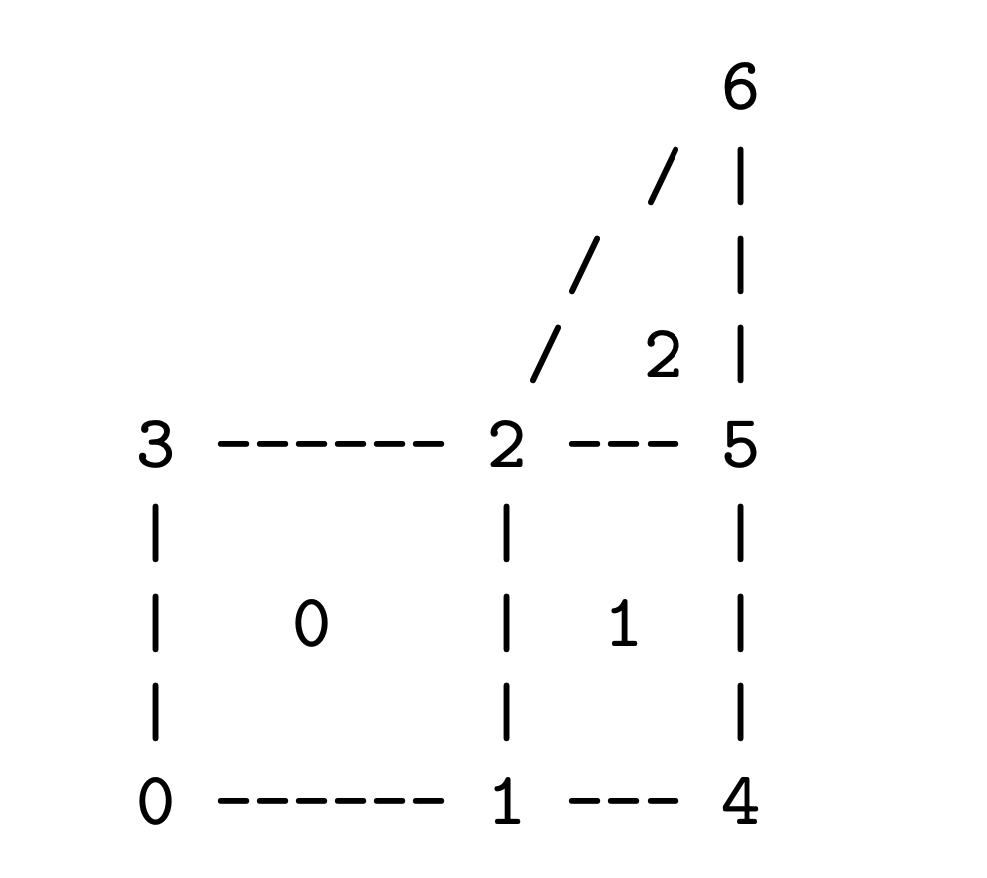
\includegraphics[width=5cm]{assets/example.png}
    \caption{Classic example of mesh with 2 quadrangles and 1 triangle}
    \label{fig:classic_example}
\end{figure}
\begin{figure}[H]
    \centering
    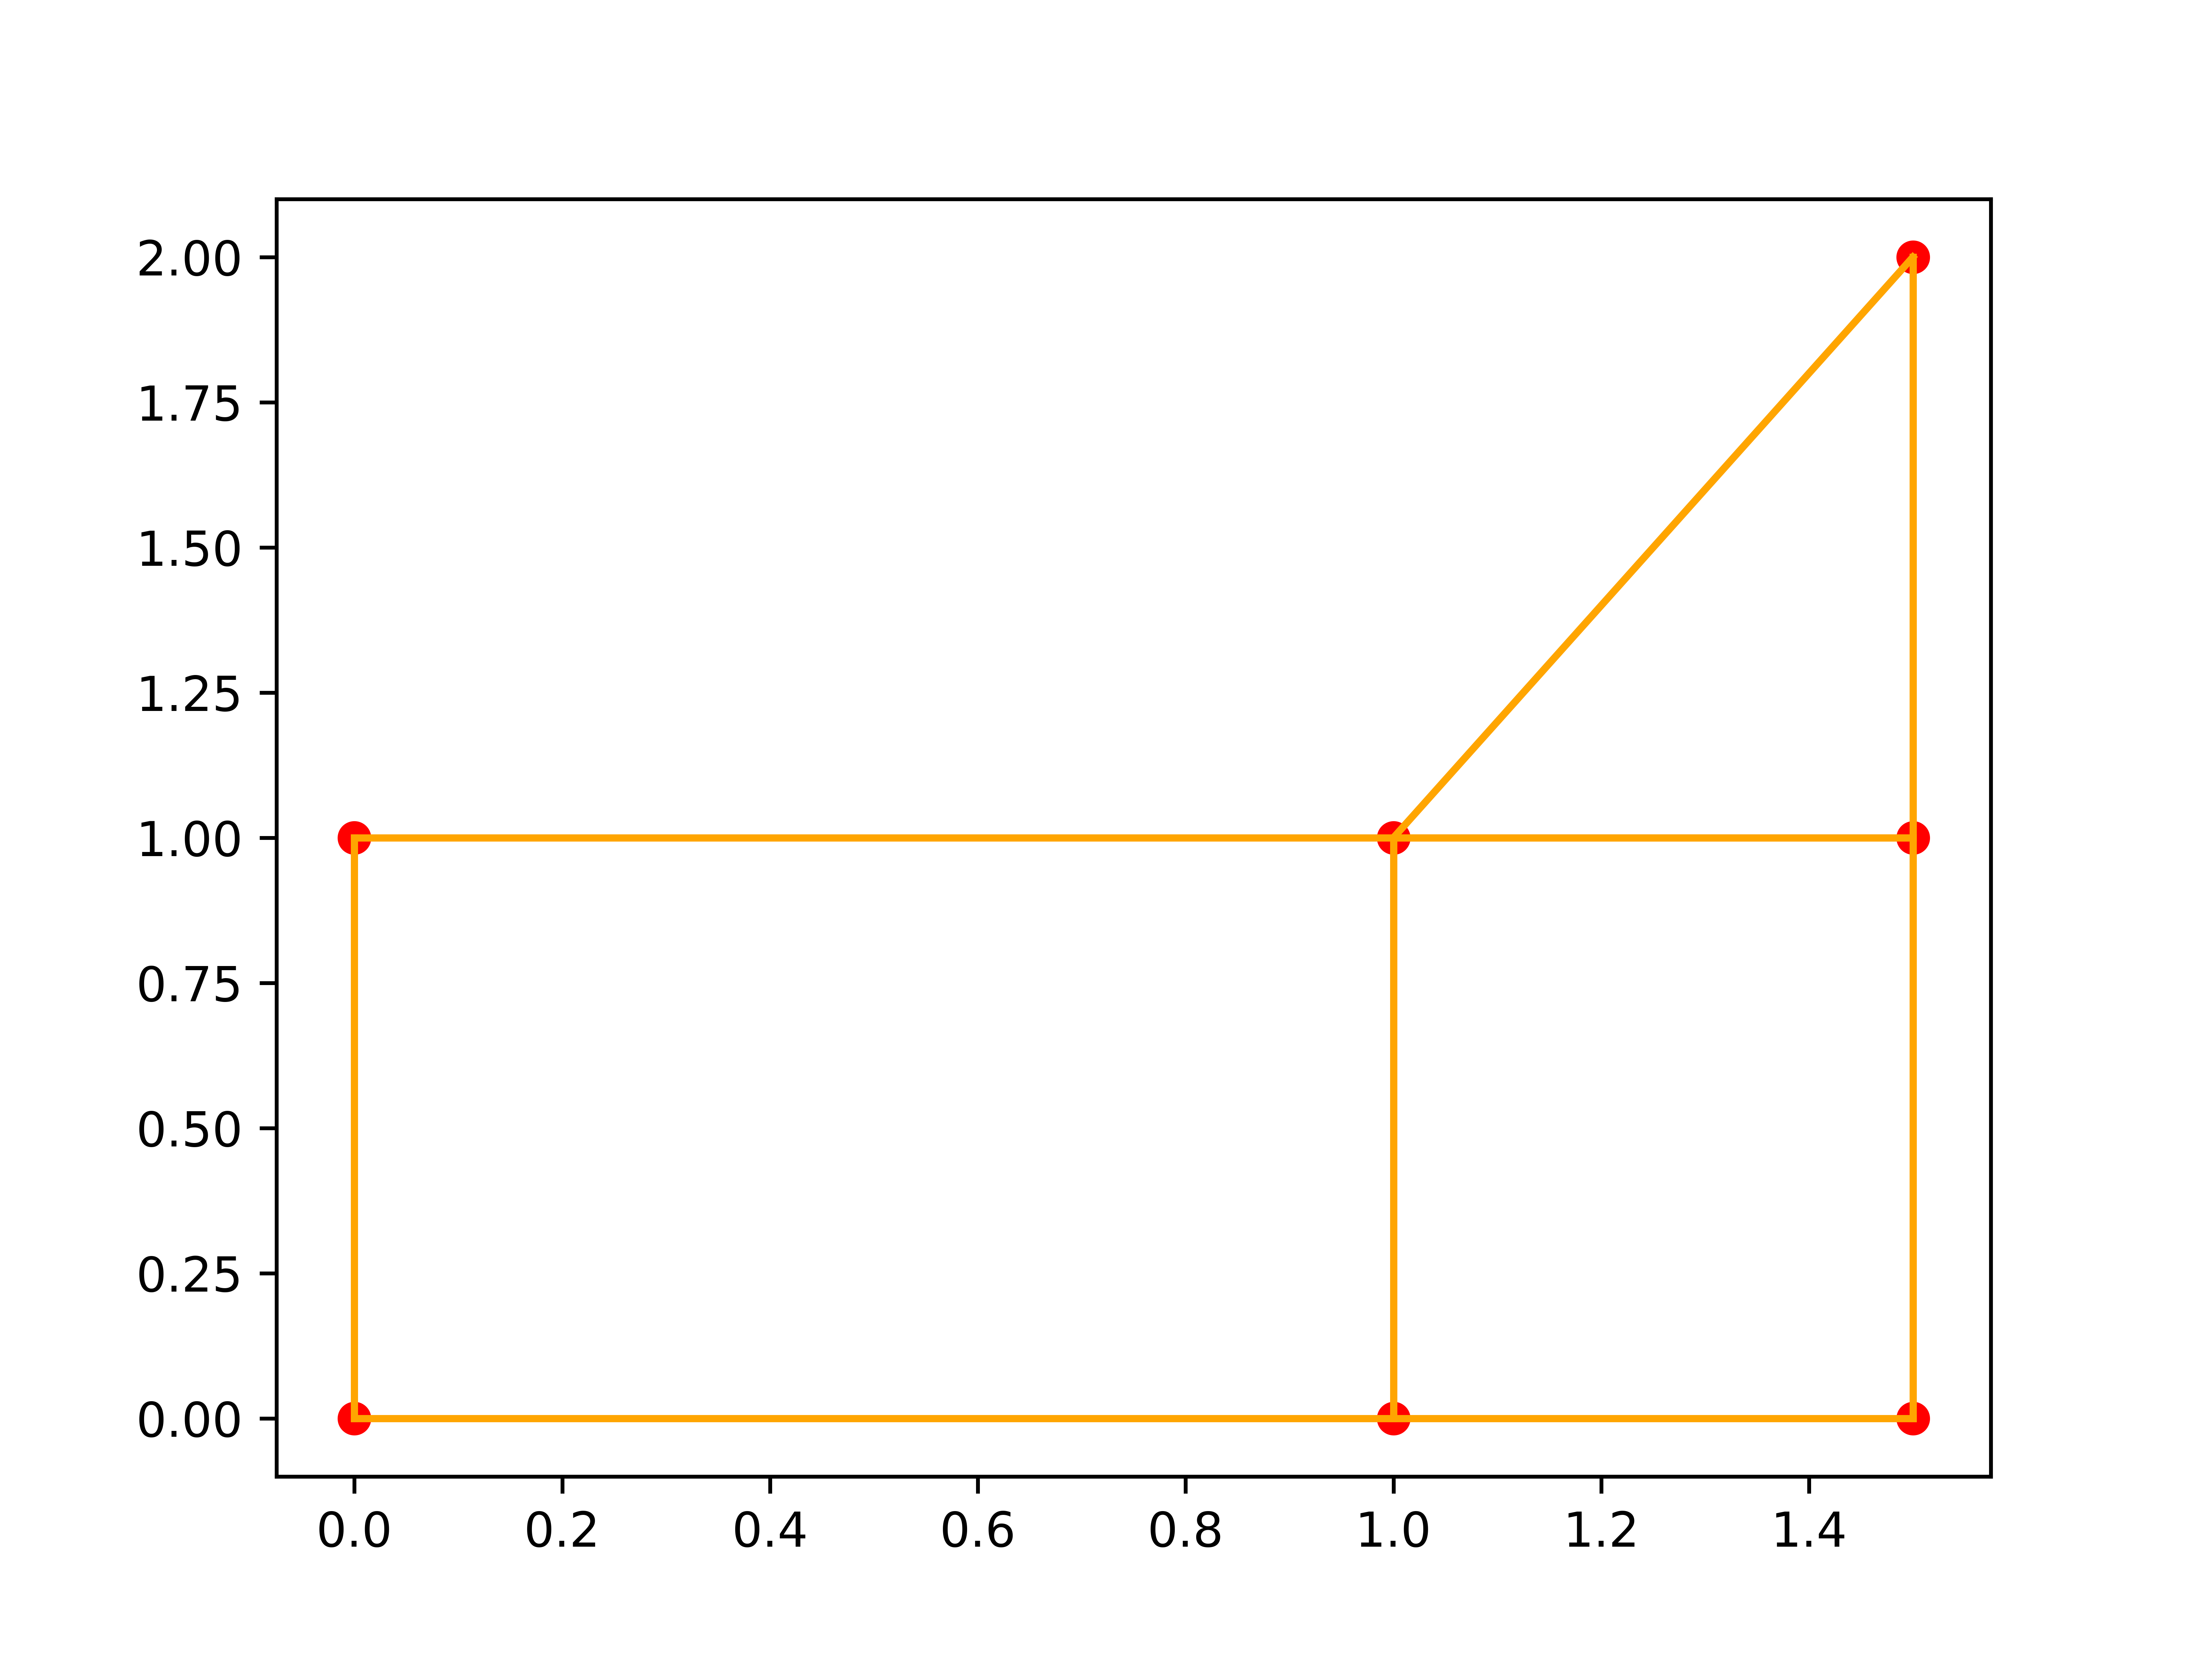
\includegraphics[width=10cm]{assets/plot.png}
    \caption{Plot of the classic example in Figure 1 using the plotting functions}
    \label{fig:plot_classic_example}
\end{figure}
\noindent Last but not least, during the courses one function to compute the arrays \texttt{node2elems} and \texttt{p\_node2elems} was given. This function is \texttt{build\_node2elems} and works with the compressed sparse row (CSR) date storage system. Knowing that, it is normally possible to understand all this report.

\section{Modifying the mesh}

\subsection{Question 7: Adding and removing nodes and elements to the mesh}

The first thing to do when you have a mesh is to be able to manipulate it. This begins by adding and removing nodes and elements.\\ \\
The first two functions \texttt{add\_elem\_to\_mesh} and \texttt{add\_node\_to\_mesh} are quick to do. There is no re-indexing and we just need to add points. These are simply done in one line by the functions \texttt{np.append(array, element to append)}.\\ \\
Here is a test of theses functions after having used the 2 commands:\\
\texttt{node\_coords, p\_elem2nodes, elem2nodes = add\_node\_to\_mesh(node\_coords, p\_elem2nodes, elem2nodes, np.array([[1, 2, 0]]))},\\
\texttt{node\_coords, p\_elem2nodes, elem2nodes = add\_elem\_to\_mesh(node\_coords, p\_elem2nodes, elem2nodes, np.array([2, 5, 6, 7]))}.
\begin{figure}[H]
    \centering
    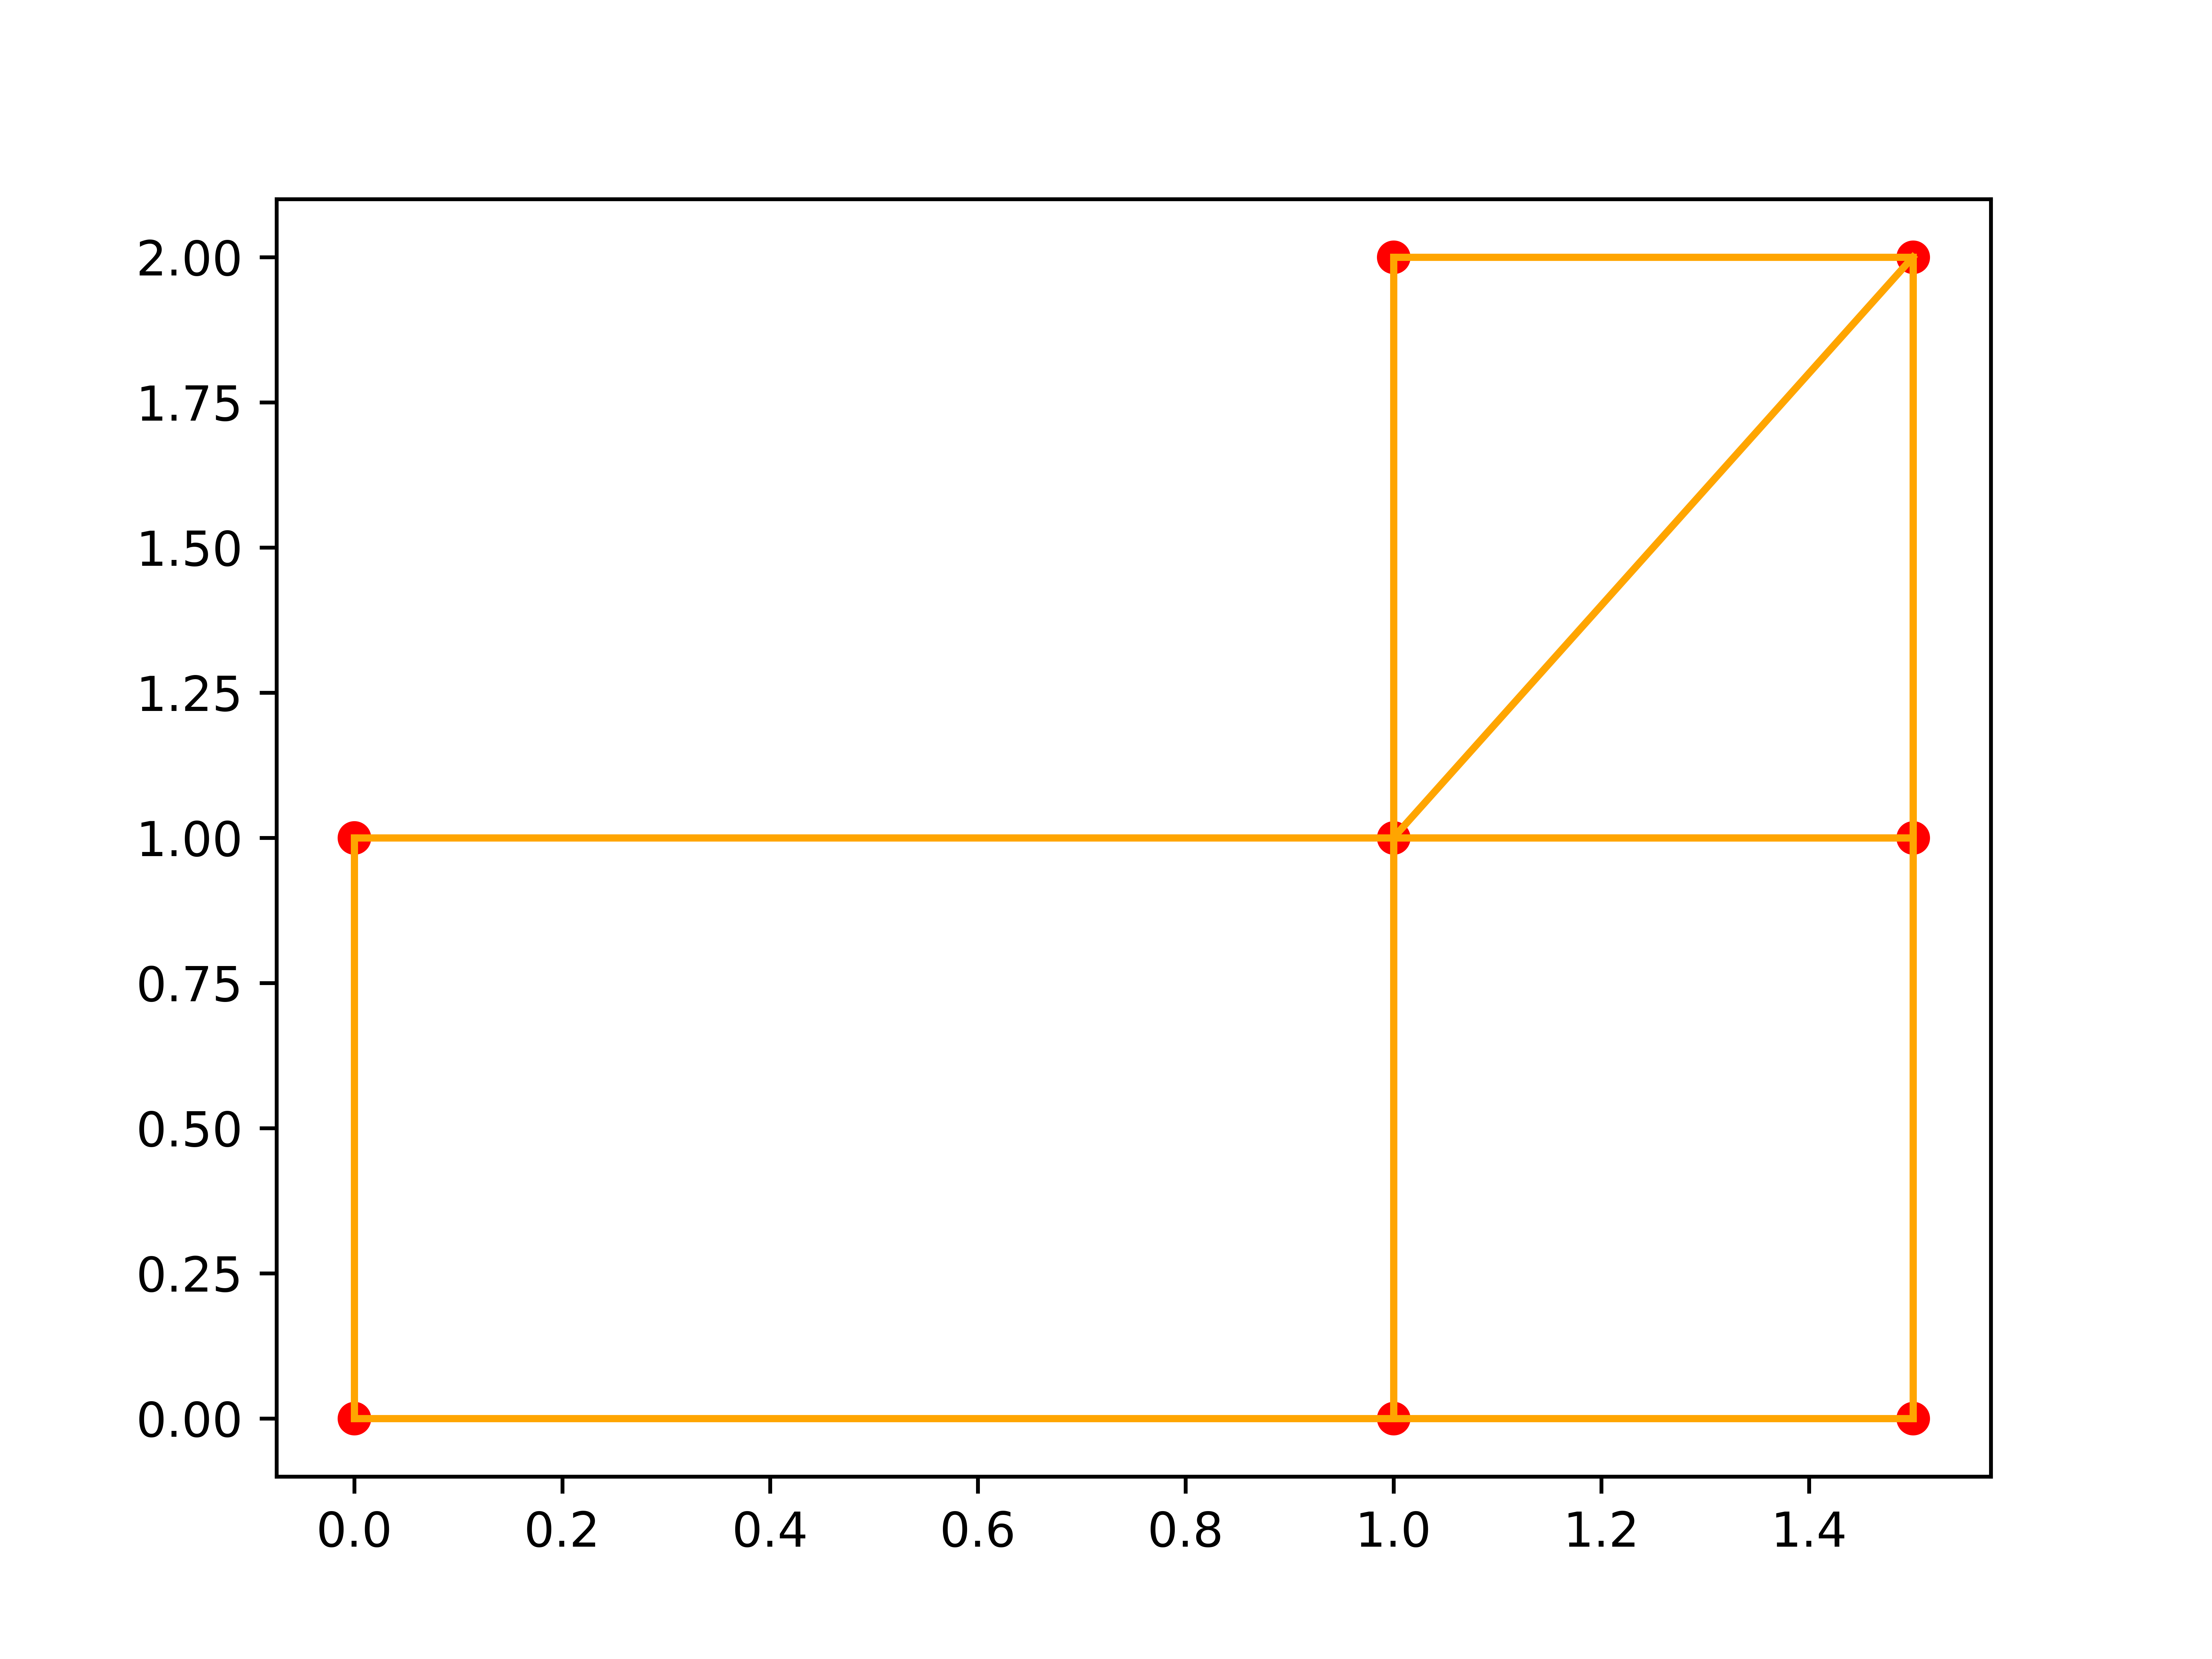
\includegraphics[width=10cm]{assets/q6_1.png}
    \caption{Plot of the classic example with one more node and one more element}
    \label{fig:plot_classic_example}
\end{figure}
\noindent Then, there is the complex part. We start by doing \texttt{remove\_elem\_to\_mesh} since it is sure that there is just one element to remove. This constant piece of information is very useful because it shortens the algorithm. This function takes as the three classic arrays and the id of the element of to remove as arguments.\\
Here is how the function works:
\begin{enumerate}
    \item Collecting the indexes of the points which only belong to the point to remove;
    \item Delete the points of the element to remove in \texttt{elem2nodes};
    \item Changing \texttt{p\_elem2nodes} by removing \texttt{p\_elem2nodes[elemid]} and shifting the values after by the number of nodes we have removed in \texttt{elem2nodes};
    \item At this point \texttt{node\_coords}, \texttt{elem2nodes} and \texttt{p\_elem2nodes} are "correct". But there may exist some orphan points in \texttt{node\_coords} which belong to zero element. We have their index thanks to the first step, so we remove them from \texttt{node\_coords} and then we change the values of the indexes in \texttt{elem2nodes} to make it correspond with the new \texttt{node\_coords}.
\end{enumerate}
For \texttt{remove\_node\_to\_mesh}, I used the previous function \texttt{remove\_elem\_to\_mesh}. Firstly, I start by collecting the indexes of the element in which the node belongs. Then, in the hypothetical case that the node belongs to $0$ element, we do the same with the previous function: we remove the point from \texttt{node\_coords} and then we change the values of the indexes in \texttt{elem2nodes} to make it correspond with the new \texttt{node\_coords}. \\
In the other case, we just apply the function \texttt{remove\_node\_to\_mesh} with every elements to whose the point belongs. Since \texttt{remove\_node\_to\_mesh} removes the orphan points, the node to remove, its elements and the points that became orphan are removed.\\ \\
We test these functions with the commands:\\
\texttt{node\_coords, p\_elem2nodes, elem2nodes = remove\_node\_to\_mesh(node\_coords, p\_elem2nodes, elem2nodes, 0)} for the Figure 4,
\texttt{node\_coords, p\_elem2nodes, elem2nodes = remove\_elem\_to\_mesh(node\_coords, p\_elem2nodes, elem2nodes, 2)} for the Figure 5.
\begin{figure}[H]
    \centering
    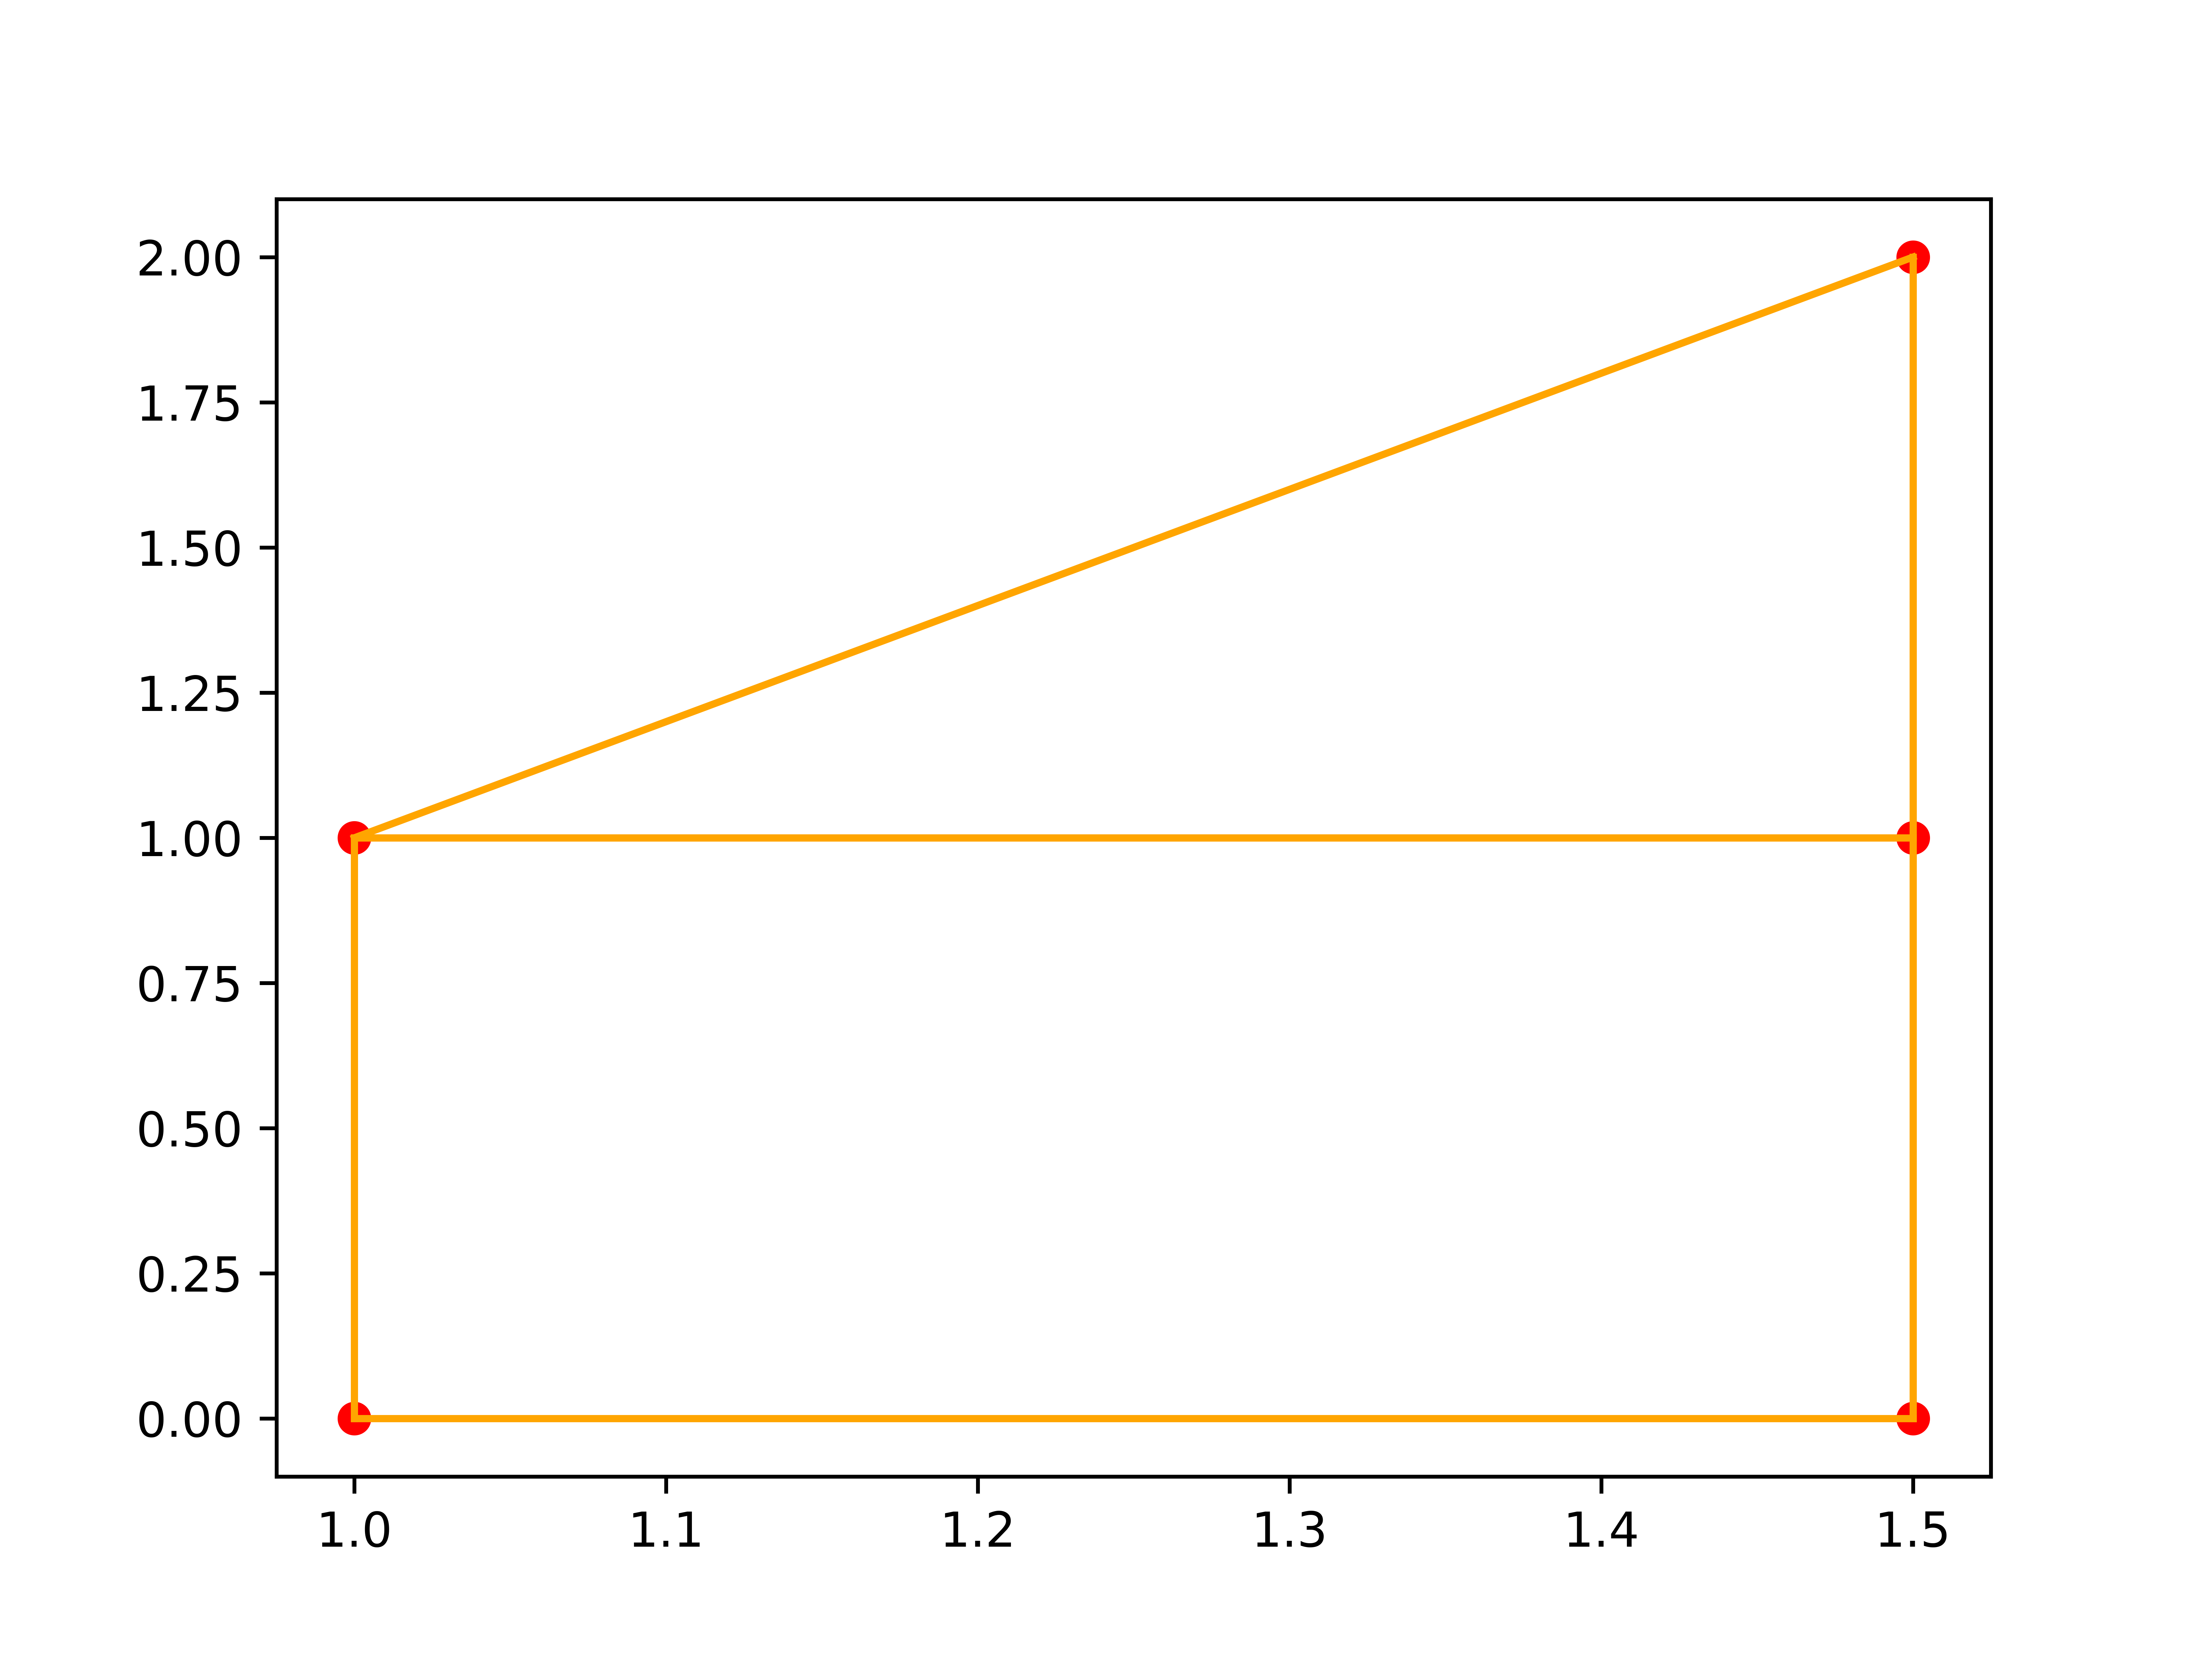
\includegraphics[width=10cm]{assets/q6_2.png}
    \caption{Plot of the classic example with the node $0$ removed}
    \label{fig:plot_classic_example}
\end{figure}
\begin{figure}[H]
    \centering
    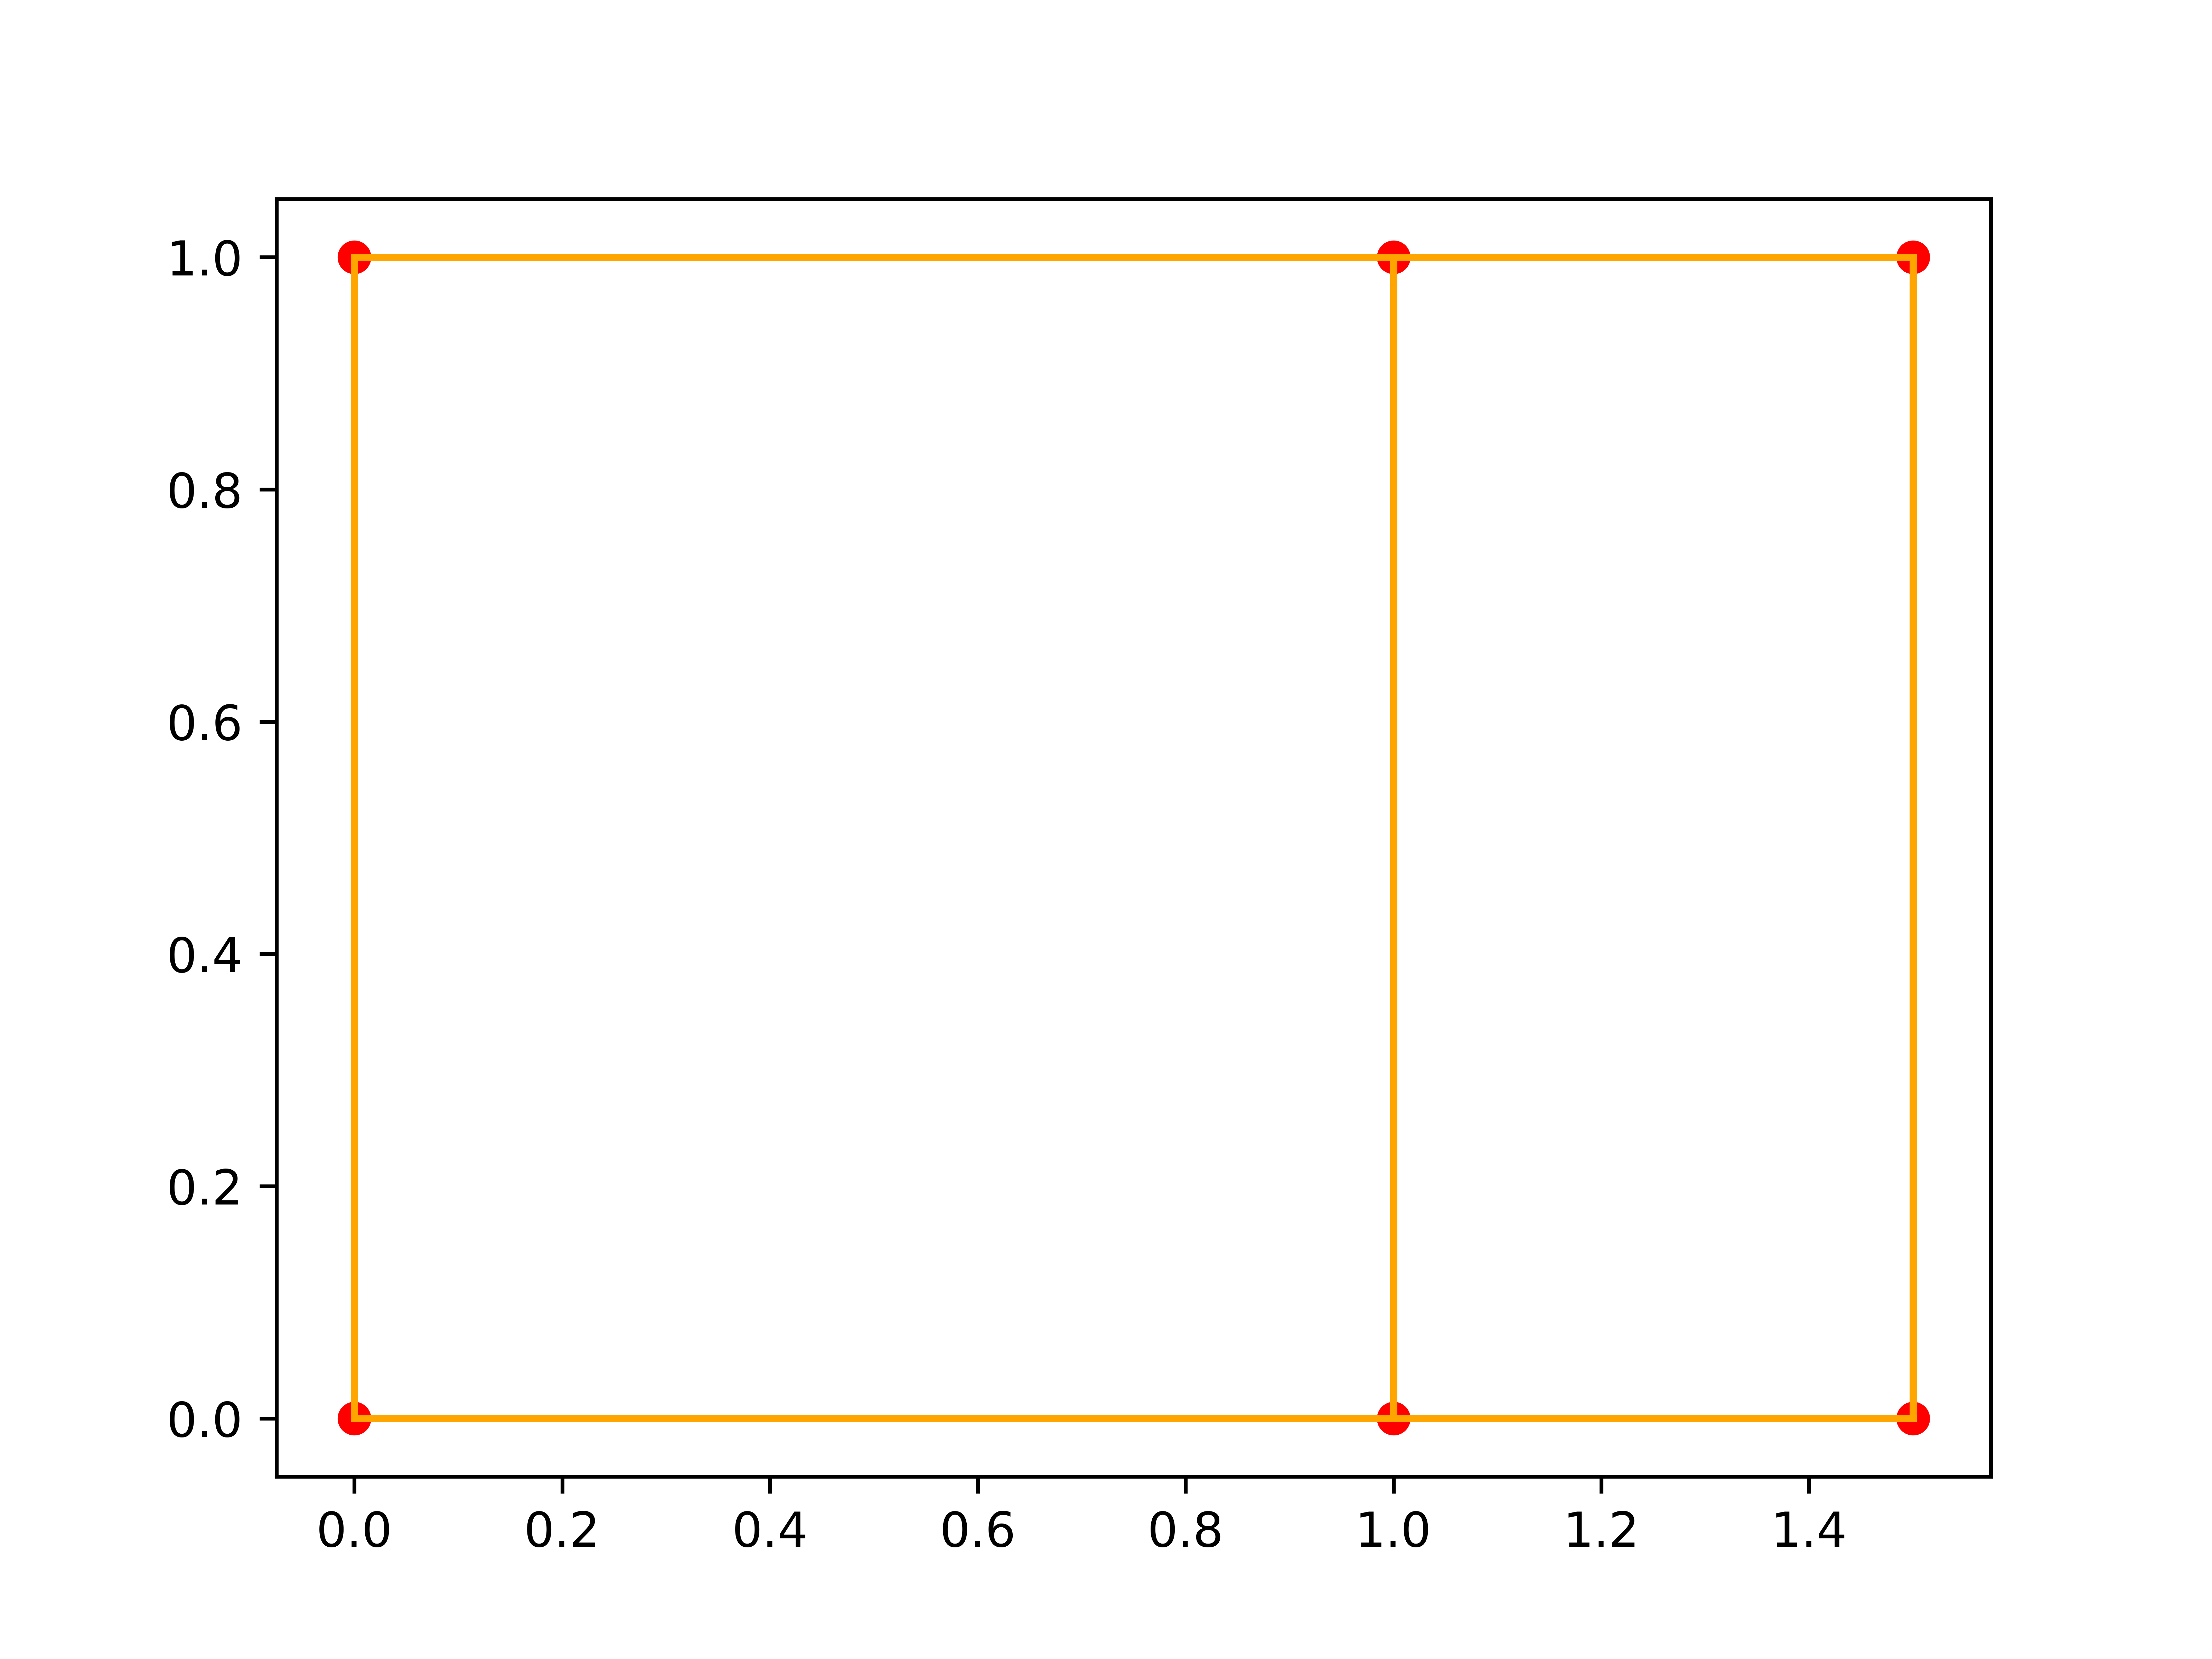
\includegraphics[width=10cm]{assets/q6_3.png}
    \caption{Plot of the classic example with the element $2$ removed}
    \label{fig:plot_classic_example}
\end{figure}

\section{Analyzing and calculating mesh quality}

\subsection{Question 1: Aspect ratio calculation}

\hspace{0.8cm} The aspect ratio is a quality metric for the quality of elements in a mesh. Its formula depends on the shape of the element. If it is a triangle, then the formula is $$\displaystyle Q = \alpha \frac{h_{max}}{\rho}$$ where $\alpha = \displaystyle \frac{\sqrt{3}}{6}$, $h_{max}$ is the longest edge of the triangle and $\rho$ is the radius of the inscribed circle. To compute $\rho$ we can use the formula: $$\displaystyle \rho = \sqrt{\frac{(s-a)(s-b)(s-c)}{s}} \text{ with } s= \frac{1}{2}(a + b+ c).$$ 
Something interesting is that the aspect ratio for triangles is greater or equal to $1$, and the equality case holds for equilateral triangle. The more the triangle will be "degenerated", for example with a very large angle, the more the aspect ratio will big.\\ \\
For quadrangles, the formula changes and becomes: $$\displaystyle Q = 1 - \frac{\displaystyle \sum_{i=1}^{4} |\bm{e_i} \bm{e_{i+1 \text{ mod 4}}}|}{4}$$ where $\bm{e_i}$ is the elementary vector supporting each side of the quadrangle. Now we remark that the aspect is between $0$ and $1$, and is equal to $1$ for a rectangle. So the more the quadrangle is degenerated, the more the aspect ratio will tend to $0$.\\ \\
To compute it we simply have to copy the formulas above. The function which does it is \texttt{compute\_aspect\_ratio}. To test the function, we compute the aspect ratio of the elements in the classic example in introduction. I found: $$Q_0 = 1,0; Q_1 =1,0; Q_2 = 1,69$$ where $Q_i$ is the aspect ratio of element $i$.

\subsection{Question 2: Length factor calculation}

\hspace{0.8cm} The length factor is one other metric to class the quality of elements in a mesh. The formula is the same whatever is the number sides that the element has. It is: $$\displaystyle E = \frac{h_{min}}{h_{medium}}.$$
The function that computes the length factor is \texttt{compute\_length\_factor}. We also test it on the classic example. I obtain: $$E_0 = 1,0 ; E_2 = 0,66 ; E_2 = 0,573$$ where $E_i$ is the edge length factor of element $i$.

\subsection{Question 4: Analysis of the mesh and diagrams}

\hspace{0.8cm} For the analysis of the mesh we need to compute the edge length factor and the aspect ratio of every elements in the mesh. In order to have quantity always between $0$ and $1$, we will take the inverse of the aspect ratio that we know for triangles. So the new formula will be: $$Q' = \displaystyle \frac{1}{Q} = \frac{\rho}{\alpha h_{max}}.$$
Know in every case, the more the quantity tend to $1$, the more the mesh is structured and regular. Then we create a histogram and we plot it thanks to \texttt{np.hist} and \texttt{matplotlib.pyplot.stairs}. The function which does this is \texttt{analysis\_of\_the\_mesh}. For the tests, there will be shown after question 3 because with the classic example it is not interesting since there is not enough nodes.

\section{Controlling mesh data}

This part is really about seeing how it is possible to use mesh data and to change it.

\subsection{Question 3: Shifting internal nodes}

It is asked to shift the internal nodes knowing already the indexes of the nodes on the border. The function which does this is \texttt{shift\_internal\_nodes}. This function starts to determine what is the minimal length of all the sides of all the elements. This allows to do a shift that is not too large whatever is the size of the mesh.\\ \\
With the test in \texttt{quadrangles\_grid\_example}, we obtain this type of shift.
\begin{figure}[H]
    \centering
    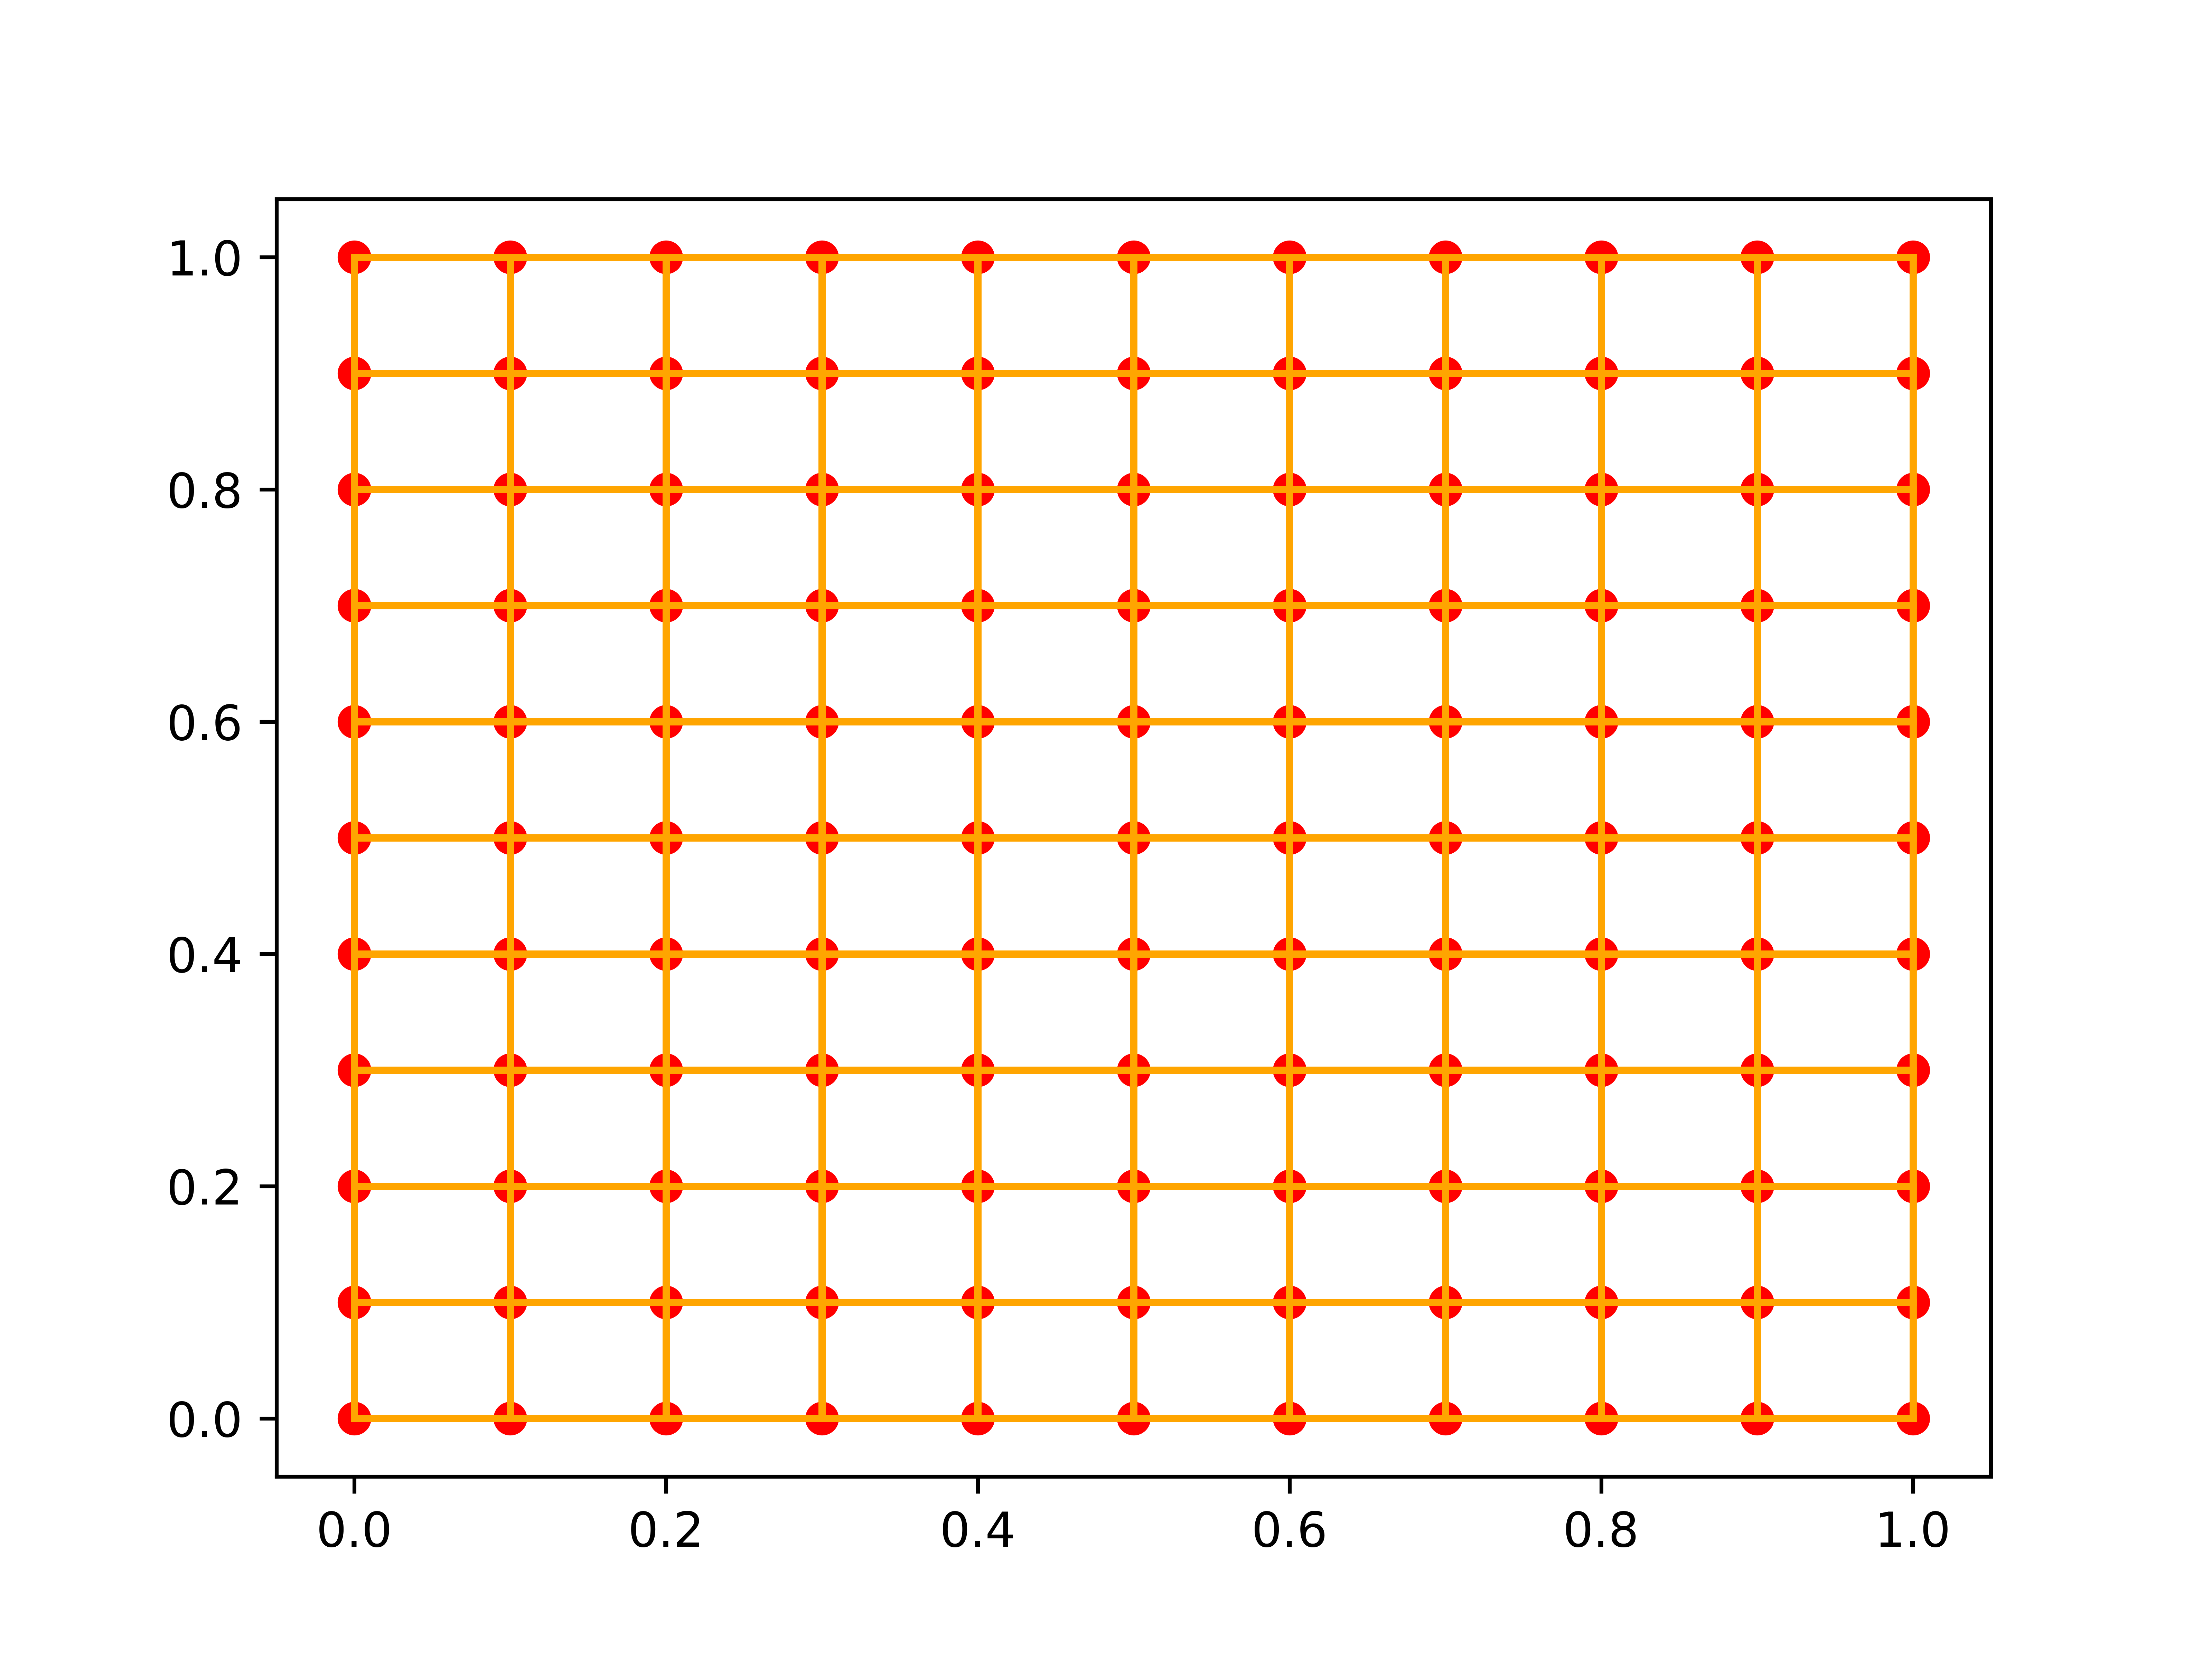
\includegraphics[width=10cm]{assets/q3_1.png}
    \caption{Original grid with quadrangles}
    \label{fig:plot_classic_example}
\end{figure}
\begin{figure}[H]
    \centering
    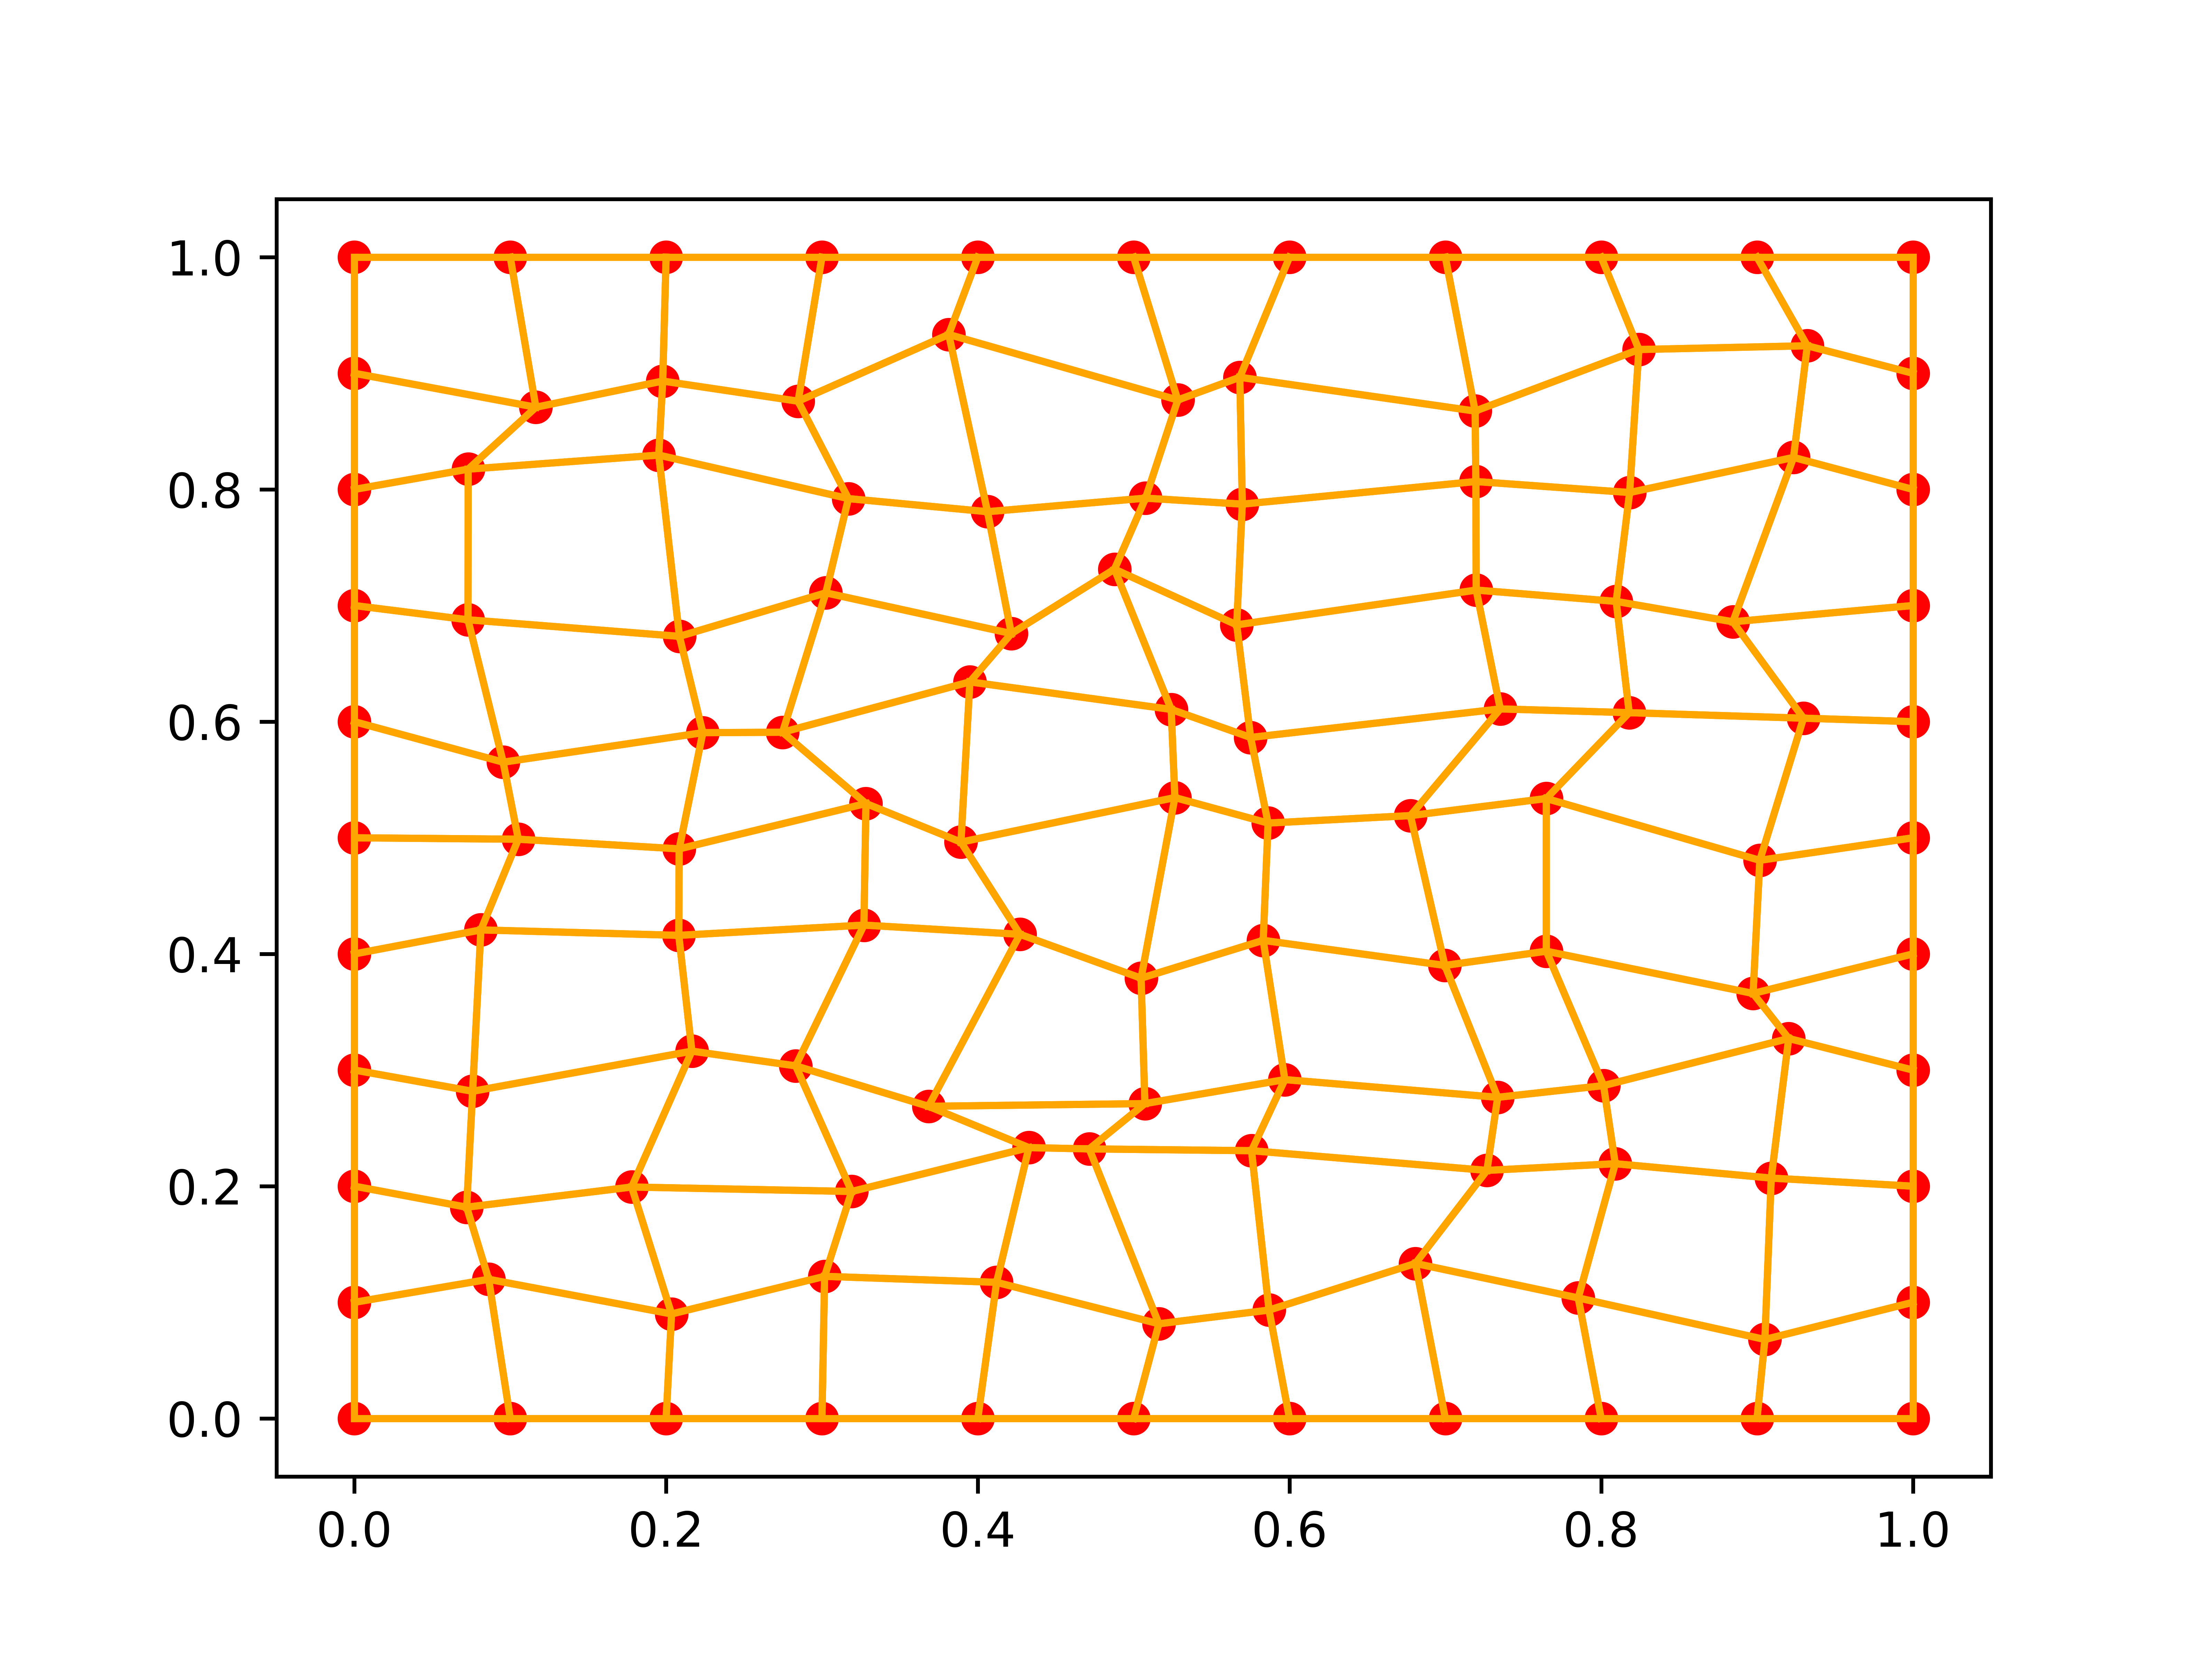
\includegraphics[width=10cm]{assets/q3_2.png}
    \caption{The same grid but with the internal nodes shifted}
    \label{fig:plot_classic_example}
\end{figure}
\noindent And for the results about the aspect ratios and the edge lengths, we obtain this.
\begin{figure}[H]
    \centering
    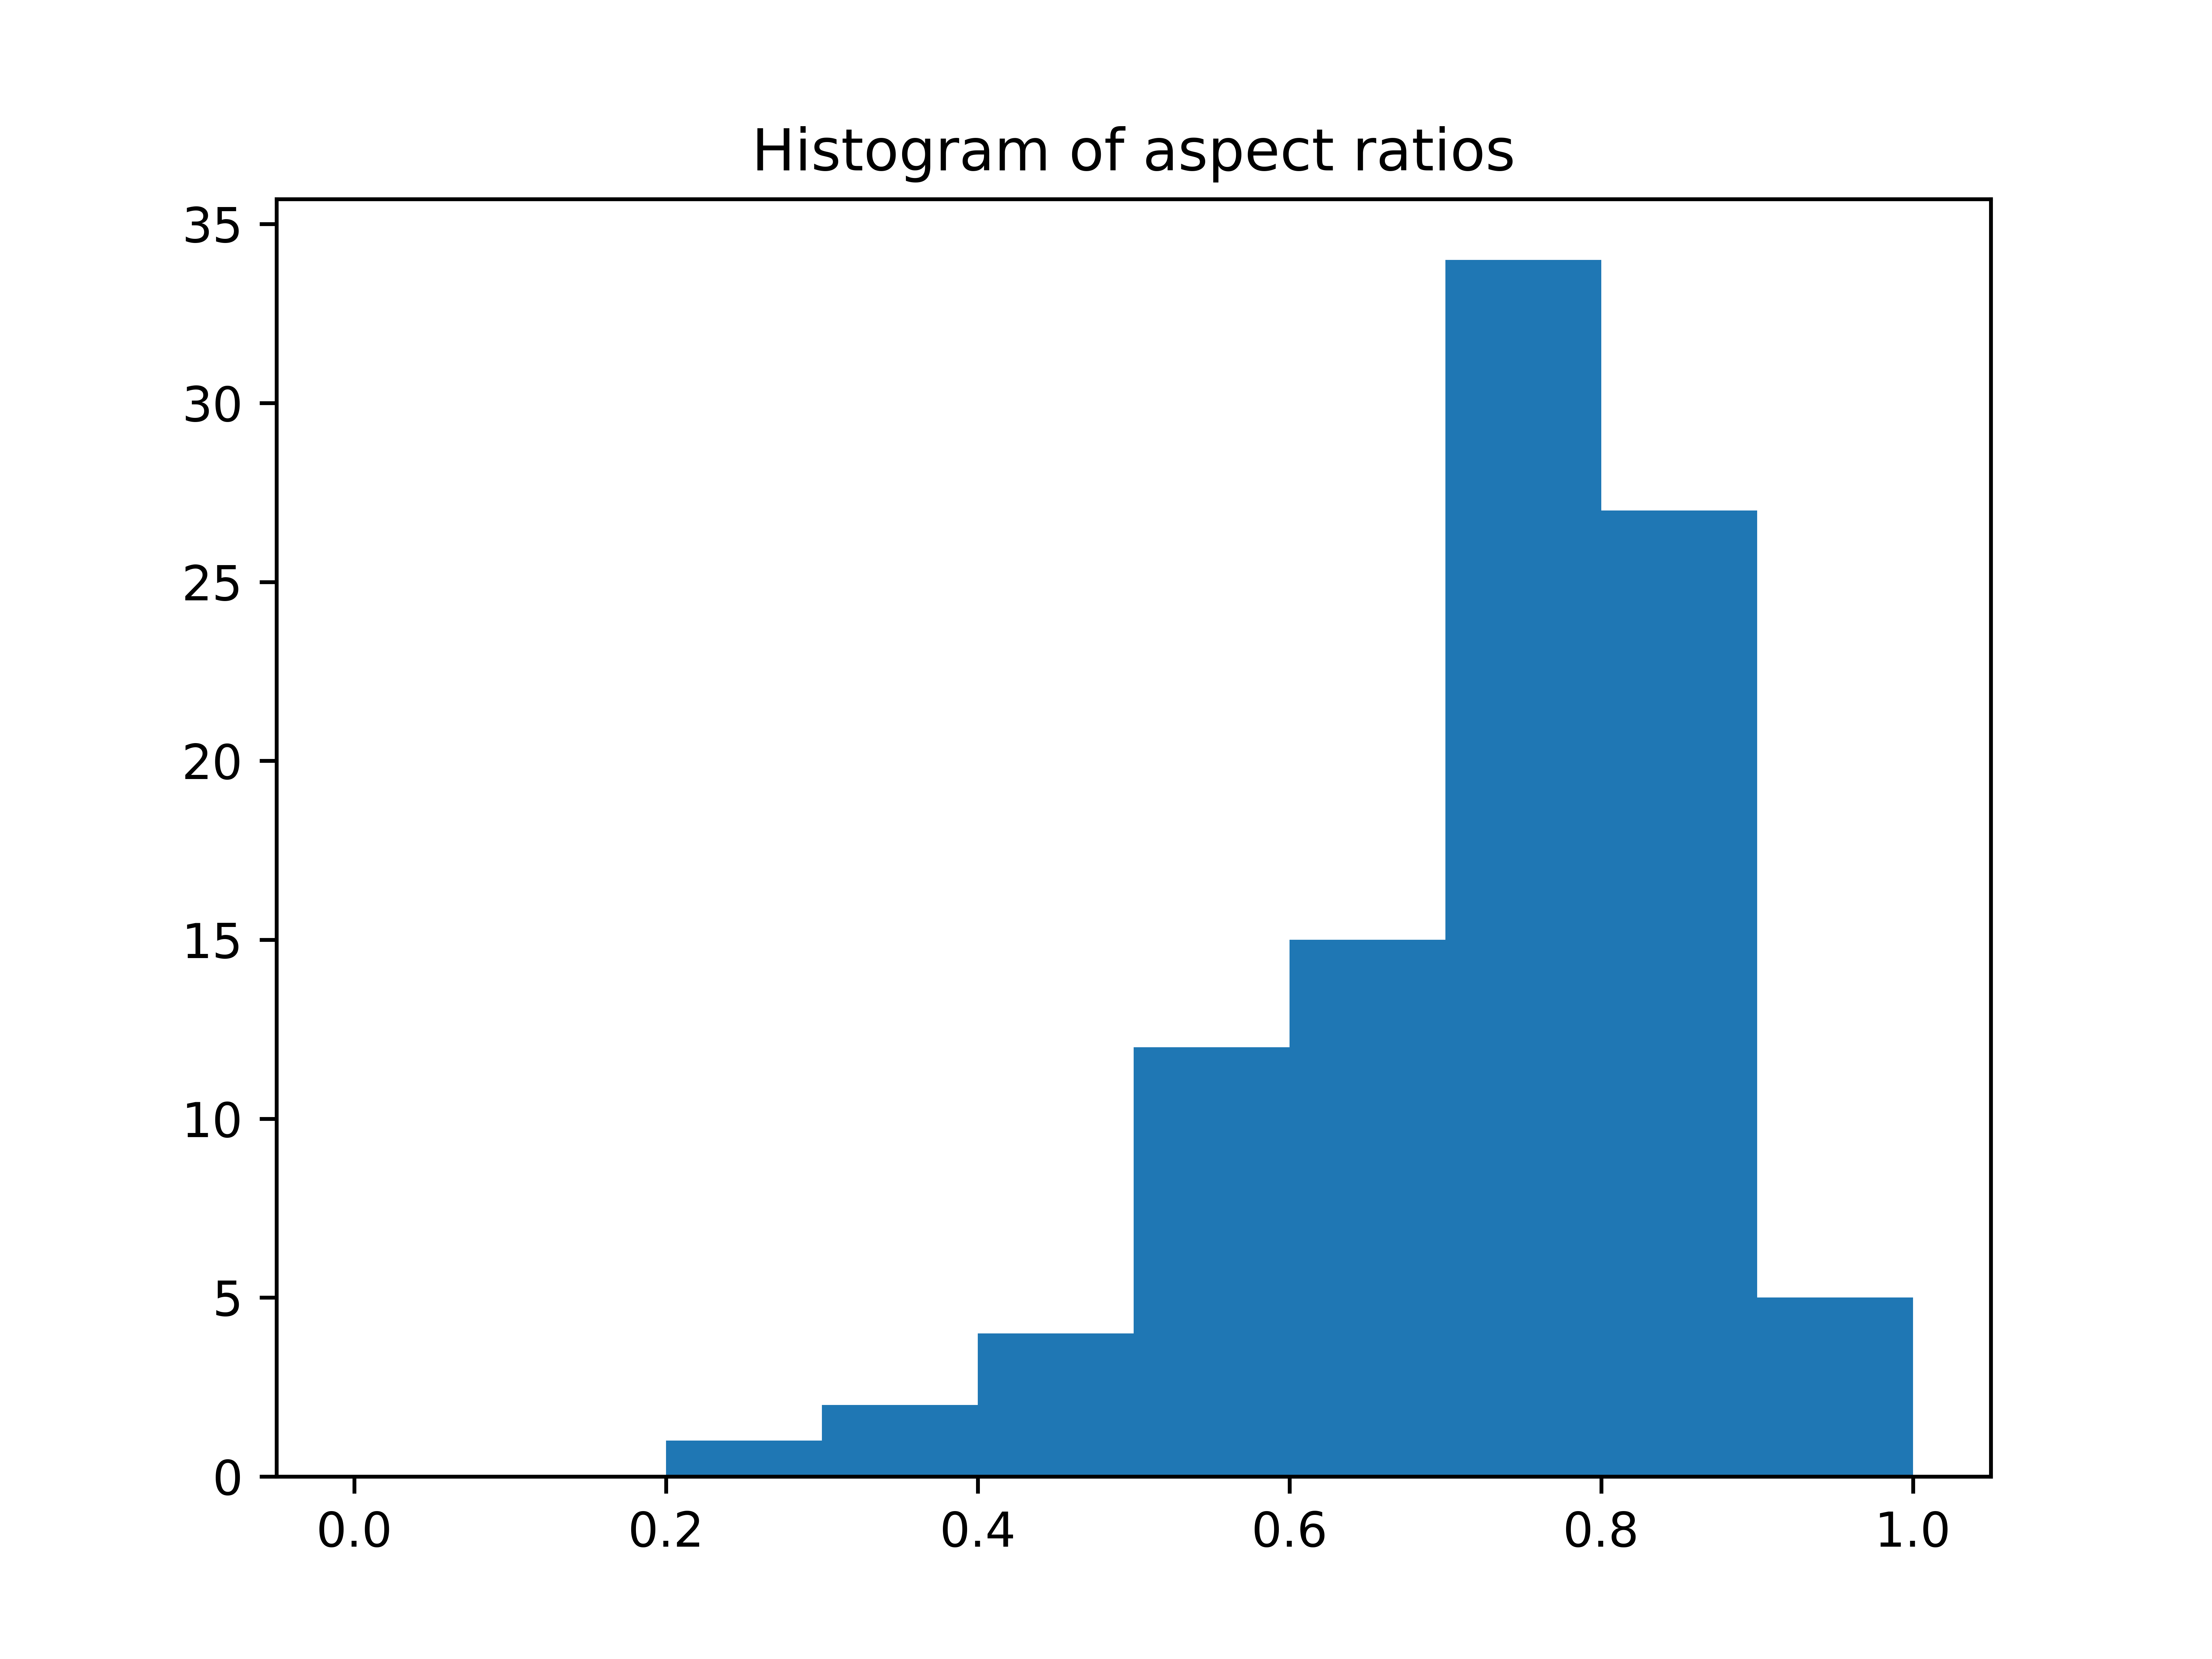
\includegraphics[width=10cm]{assets/Aspect ratios.png}
    \caption{Histogram of aspect ratios of the elements in the shifted grid just above}
    \label{fig:plot_classic_example}
\end{figure}
\begin{figure}[H]
    \centering
    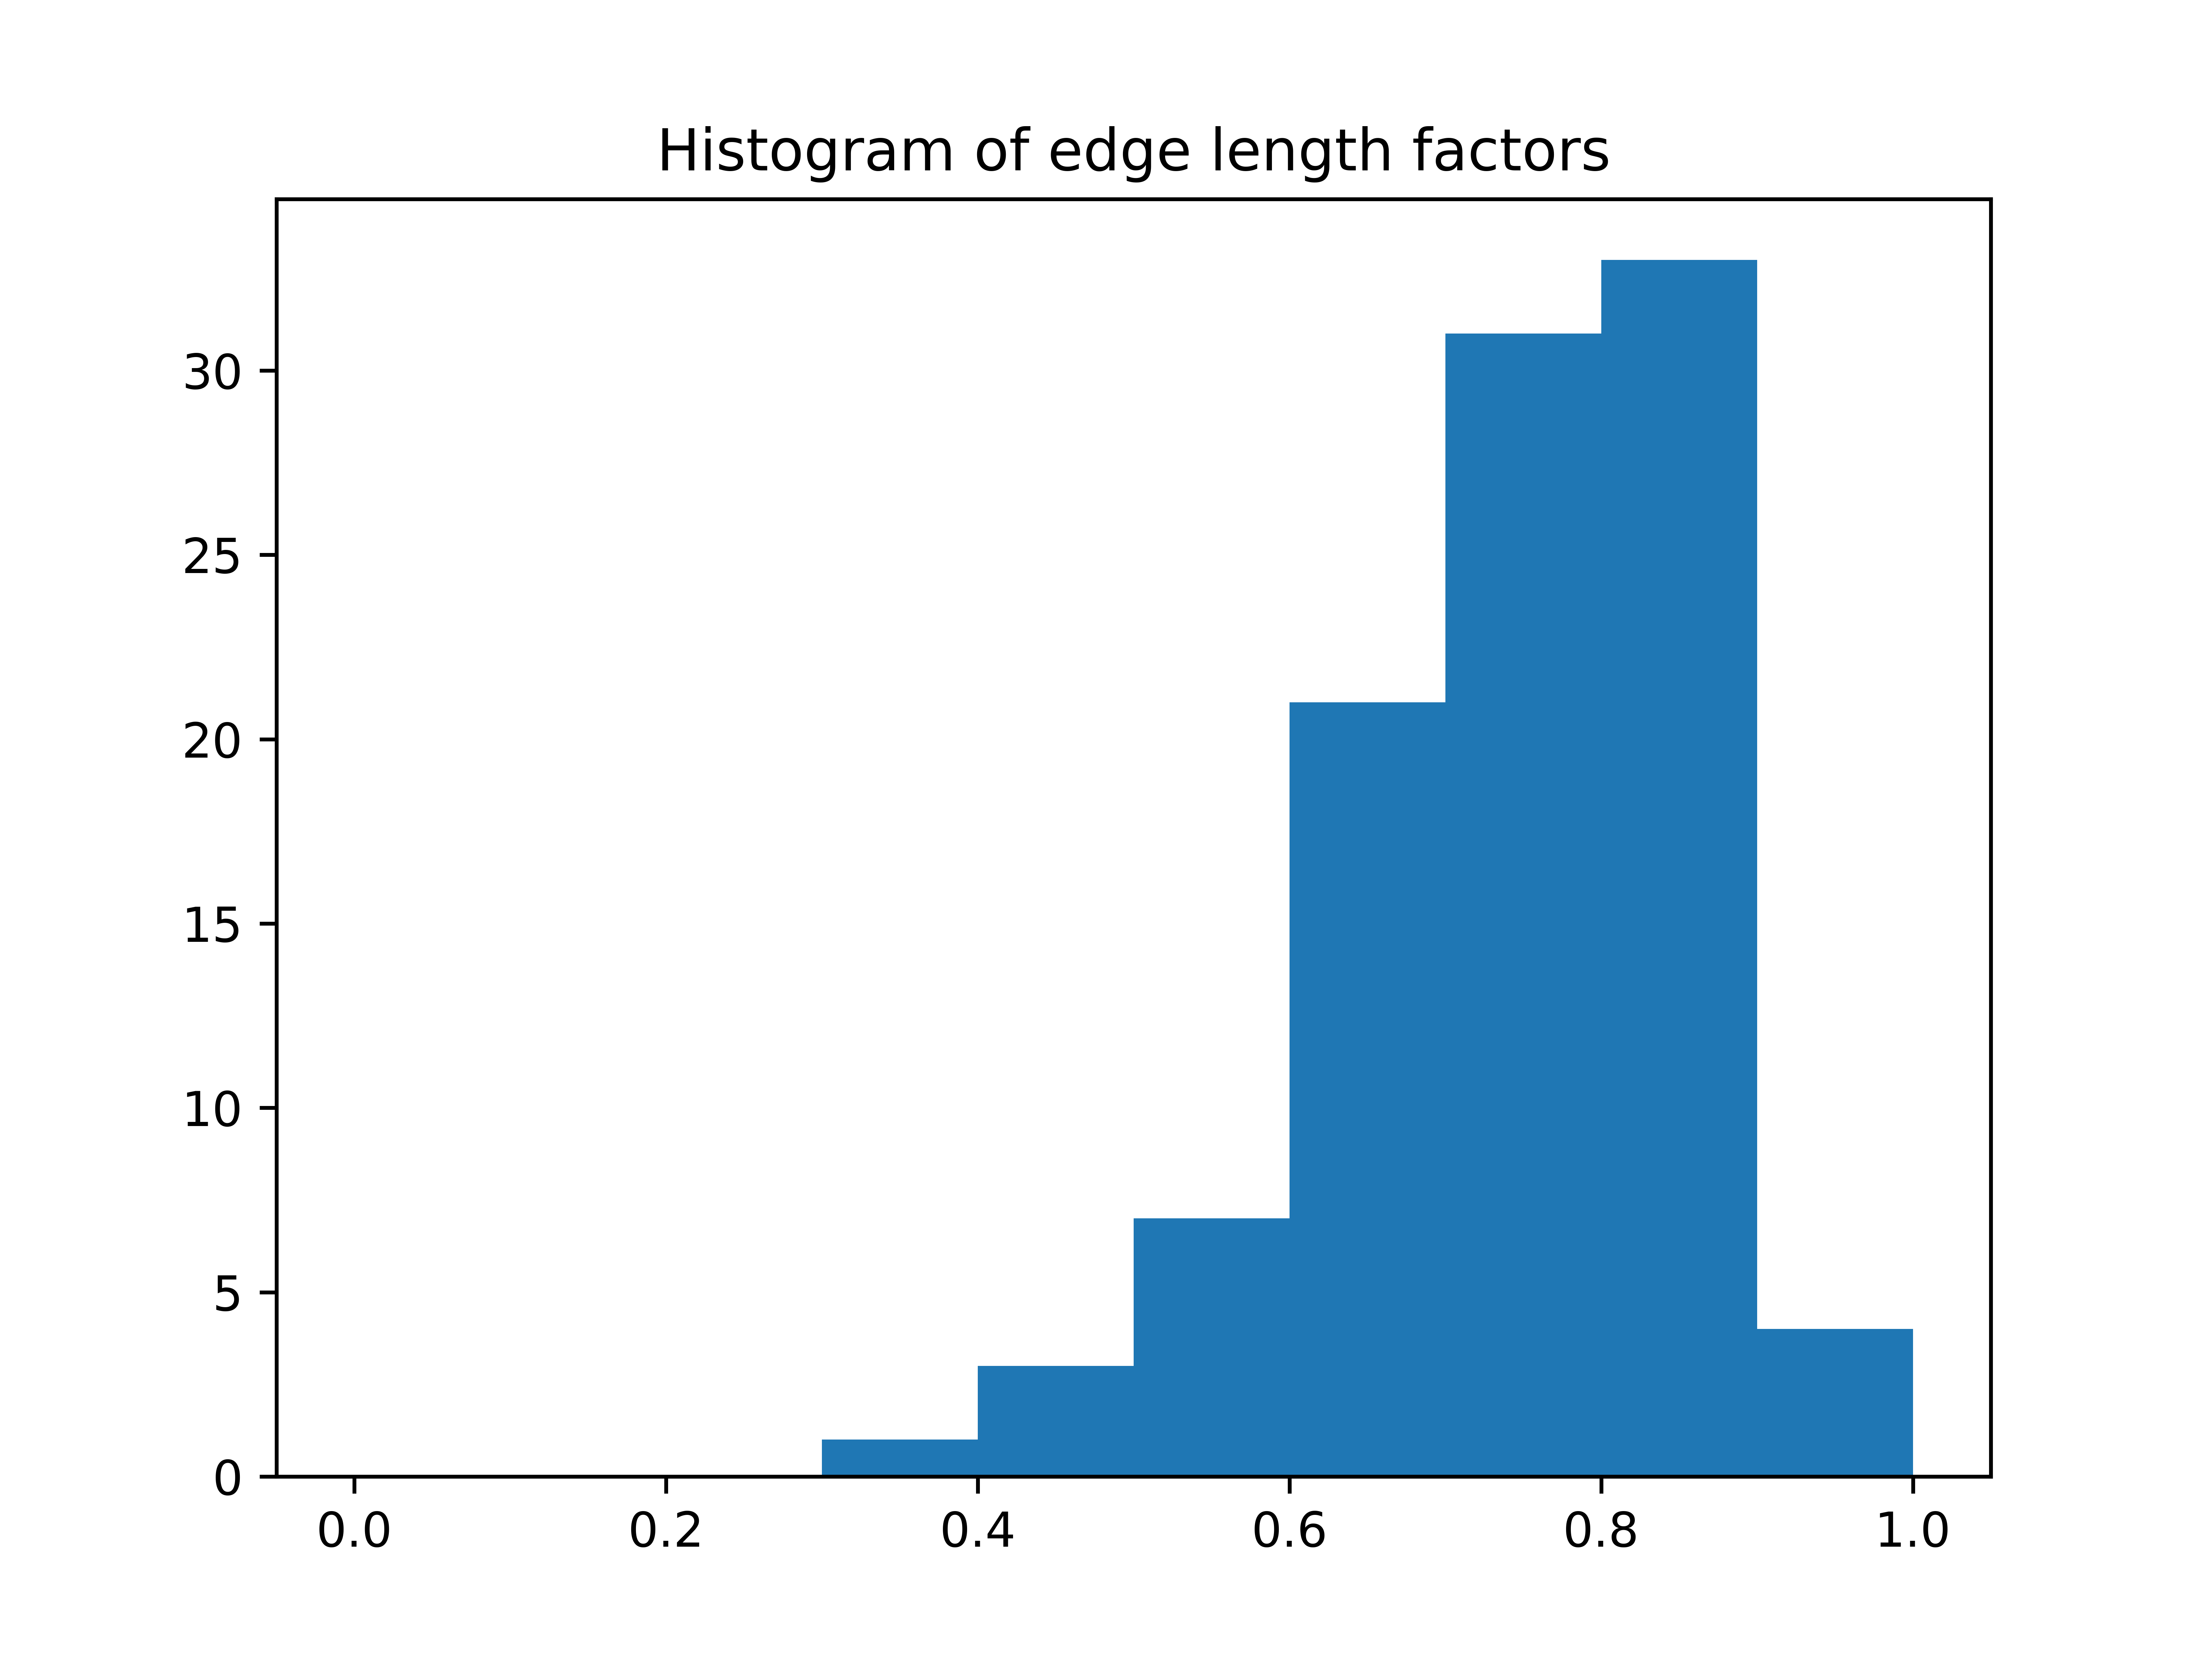
\includegraphics[width=10cm]{assets/Edge length.png}
    \caption{Histogram of edge length factors of the elements in the shifted grid just above}
    \label{fig:plot_classic_example}
\end{figure}

\subsection{Question 5: Computing barycenters of element}

This function was given during the lectures. It just computes the average of the coordinates of the nodes which belong to the element. The code is in the function \texttt{compute\_barycenter\_of\_element}.

\section{Creating fractals}

\subsection{Question 8}

Fractals are very important when it comes to controlling the acoustic waves because they can prison the waves. To create a fractal we need to repeat one pattern again and again. To make this surface constant, I chose to repeat one pattern that has a zero area (i.e. the integral of the pattern is equal to $0$).\\ \\
In my code a pattern is an array of coordinates of points that represent the one side of the fractal between points $(0, 0)$ and $(0,1)$. Then, for each side where I need to apply the pattern I take the extrema of the sides and I apply a rotation, a homothety and a translation to have the coordinates of the points to insert. It gives this:
\begin{figure}[H]
    \centering
    \includegraphics[width=12cm]{assets/n=3 all_steps dpi=1500.png}
    \caption{Fractal obtained by starting with a square and a squared pattern}
    \label{fig:plot_classic_example}
\end{figure}
\noindent For the meshing of these fractals, i am currently working on the Rupper's algorithm that creates good mesh whatever is the form. I have already done the constrained Delaunay algorithm.

\end{document}